% Options for packages loaded elsewhere
\PassOptionsToPackage{unicode}{hyperref}
\PassOptionsToPackage{hyphens}{url}
%
\documentclass[
]{book}
\usepackage{amsmath,amssymb}
\usepackage{lmodern}
\usepackage{ifxetex,ifluatex}
\ifnum 0\ifxetex 1\fi\ifluatex 1\fi=0 % if pdftex
  \usepackage[T1]{fontenc}
  \usepackage[utf8]{inputenc}
  \usepackage{textcomp} % provide euro and other symbols
\else % if luatex or xetex
  \usepackage{unicode-math}
  \defaultfontfeatures{Scale=MatchLowercase}
  \defaultfontfeatures[\rmfamily]{Ligatures=TeX,Scale=1}
\fi
% Use upquote if available, for straight quotes in verbatim environments
\IfFileExists{upquote.sty}{\usepackage{upquote}}{}
\IfFileExists{microtype.sty}{% use microtype if available
  \usepackage[]{microtype}
  \UseMicrotypeSet[protrusion]{basicmath} % disable protrusion for tt fonts
}{}
\makeatletter
\@ifundefined{KOMAClassName}{% if non-KOMA class
  \IfFileExists{parskip.sty}{%
    \usepackage{parskip}
  }{% else
    \setlength{\parindent}{0pt}
    \setlength{\parskip}{6pt plus 2pt minus 1pt}}
}{% if KOMA class
  \KOMAoptions{parskip=half}}
\makeatother
\usepackage{xcolor}
\IfFileExists{xurl.sty}{\usepackage{xurl}}{} % add URL line breaks if available
\IfFileExists{bookmark.sty}{\usepackage{bookmark}}{\usepackage{hyperref}}
\hypersetup{
  pdftitle={Cresko Laboratory Manual},
  pdfauthor={Cresko Lab},
  hidelinks,
  pdfcreator={LaTeX via pandoc}}
\urlstyle{same} % disable monospaced font for URLs
\usepackage{longtable,booktabs,array}
\usepackage{calc} % for calculating minipage widths
% Correct order of tables after \paragraph or \subparagraph
\usepackage{etoolbox}
\makeatletter
\patchcmd\longtable{\par}{\if@noskipsec\mbox{}\fi\par}{}{}
\makeatother
% Allow footnotes in longtable head/foot
\IfFileExists{footnotehyper.sty}{\usepackage{footnotehyper}}{\usepackage{footnote}}
\makesavenoteenv{longtable}
\usepackage{graphicx}
\makeatletter
\def\maxwidth{\ifdim\Gin@nat@width>\linewidth\linewidth\else\Gin@nat@width\fi}
\def\maxheight{\ifdim\Gin@nat@height>\textheight\textheight\else\Gin@nat@height\fi}
\makeatother
% Scale images if necessary, so that they will not overflow the page
% margins by default, and it is still possible to overwrite the defaults
% using explicit options in \includegraphics[width, height, ...]{}
\setkeys{Gin}{width=\maxwidth,height=\maxheight,keepaspectratio}
% Set default figure placement to htbp
\makeatletter
\def\fps@figure{htbp}
\makeatother
\setlength{\emergencystretch}{3em} % prevent overfull lines
\providecommand{\tightlist}{%
  \setlength{\itemsep}{0pt}\setlength{\parskip}{0pt}}
\setcounter{secnumdepth}{5}
\usepackage{booktabs}
\usepackage{amsthm}
\makeatletter
\def\thm@space@setup{%
  \thm@preskip=8pt plus 2pt minus 4pt
  \thm@postskip=\thm@preskip
}
\makeatother
\ifluatex
  \usepackage{selnolig}  % disable illegal ligatures
\fi
\usepackage[]{natbib}
\bibliographystyle{apalike}

\title{Cresko Laboratory Manual}
\author{Cresko Lab}
\date{2021-05-12}

\begin{document}
\maketitle

{
\setcounter{tocdepth}{1}
\tableofcontents
}
\hypertarget{the-cresko-lab}{%
\chapter{The Cresko Lab}\label{the-cresko-lab}}

Description of our laboratory

\hypertarget{introduction-to-the-lab}{%
\chapter{Introduction to the Lab}\label{introduction-to-the-lab}}

\begin{figure}
\centering

\includegraphics{images/Lab_logo.png}
\caption{Illustration by Dr.~Allison Fuiten}
\end{figure}

We are an intellectual community of geneticists who specializes in quantitative evolutionary genomics. Our laboratory studies the developmental genetic and genomic basis of evolution in natural populations. We use the threespine stickleback and zebrafish as the main animal models in the laboratory, as well as syngnathid. We have produced some of the first work that has helped develop stickleback into a model for dissecting the genetic basis of natural variation. We have developed genomic tools such as sequenced Restriction site Associated DNA (RAD) tags that help geneticists apply Next Generation Sequencing (NGS) technologies to biomedical and evolutionary genetic problems. These techniques allow for the efficient identification of thousands of single nucleotide polymorphisms (SNPs) throughout the genomes of models and non-model organisms. We produced the first SNP whole genome-scan for selection in the stickleback genome, and we developed novel Maximum Likelihood (ML) analytical tools for NGS data. Computational biologists and computer scientists in our team have produced software packages for genomic analyses that are used by laboratories around the world for the analysis of big data problems. Our laboratory has developed protocols, best practices, and tools for RNA-seq based transcriptomic functional analyses.

\hypertarget{mission-and-vision}{%
\chapter{Mission and Vision}\label{mission-and-vision}}

\begin{figure}
\centering
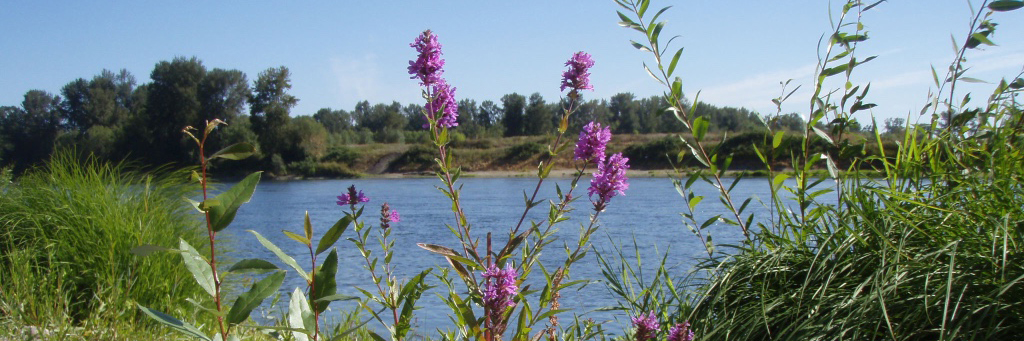
\includegraphics{images/willamette_header.jpg}
\caption{Willametter River}
\end{figure}

We describe our methods in this chapter.

\hypertarget{lab-expectations}{%
\chapter{Lab Expectations}\label{lab-expectations}}

\hypertarget{scientific-ethics-and-integrity}{%
\section{Scientific Ethics and Integrity}\label{scientific-ethics-and-integrity}}

\begin{itemize}
\tightlist
\item
  xx
\item
  xx
\item
  xx
\end{itemize}

\hypertarget{authorship-of-manuscripts}{%
\section{Authorship of Manuscripts}\label{authorship-of-manuscripts}}

\textbf{Recommended: At the start of each project, design your plan for authorship of the project so
everyone knows the expectations}

\emph{Authorship criteria}:

\begin{enumerate}
\def\labelenumi{\arabic{enumi})}
\tightlist
\item
  Makes a significant intellectual contribution to research ideas and experimental design
\end{enumerate}

OR

\begin{enumerate}
\def\labelenumi{\arabic{enumi})}
\setcounter{enumi}{1}
\tightlist
\item
  Makes a significant contribution to data acquisition, data generation, data analysis, data
  interpretation, research coordination, and/or financial support of research
\end{enumerate}

AND

\begin{enumerate}
\def\labelenumi{\arabic{enumi})}
\setcounter{enumi}{2}
\tightlist
\item
  Contributes to writing part of the manuscript, in addition to editing revisions before
  submission for publication
\end{enumerate}

AND

\begin{enumerate}
\def\labelenumi{\arabic{enumi})}
\setcounter{enumi}{3}
\tightlist
\item
  Remains involved throughout the submission and revision process until final publication
\end{enumerate}

*Research participants not meeting the criteria should be listed in the Acknowledgments
section of the final published manuscript

\emph{Authorship order}:

Generally, the person who had the most significant contribution to the project and who does
most of the writing will be the first author. In ecology, the last author is generally the PI of the
lab (although not always). The remaining authors are usually listed in their order of
contribution. However, if contributions were equivalent, then co-authors can be alphabetized
or ordered according to their time since involvement in the project.

\hypertarget{cresko-lab-safety-protocols}{%
\chapter{Cresko Lab Safety protocols}\label{cresko-lab-safety-protocols}}

\textbf{FOR YOUR OWN SAFETY AND THE SAFETY OF OTHERS, HEED THE FOLLOWING RULES!}

EMERGENCY CONTACT: dial 911 first, \emph{AND} 6-2919 (EHS) \textbar{} Mark Cell 541-505-0006

\textbf{Safety Shower, Eyewash, Fire Extinguishers.}

Eyewashes must be flushed weekly. \emph{Undergraduate research assistants are responsible for flushing the safety showers each week.} \_Each lab member is responsible for knowing the locations of safety showers and fire extinguishers in the lab. Safety showers and fire extinguishers are tested annually by EHS.

\textbf{Wear a lab coat and closed-toed shoes when working with the following chemicals:}

\begin{itemize}
\tightlist
\item
  organics (e.g.~phenol/chloroform, Trizol, DNAzol, formaldehyde, formamide, methanol)
\item
  strong acids and bases
\end{itemize}

\textbf{Wear eye protection when working with:}

\begin{itemize}
\item
  UV light (UV opaque glasses/face shield)
\item
  phenol/chloroform, strong acids/bases, and any splash hazard with anything hazardous in it.
\end{itemize}

\textbf{Wear safety gloves when working with ANY of the reagents above.}

Heed the ``one glove rule'': remove one glove when moving between rooms to avoid touching doorknobs with a contaminated glove. Note that glove materials differ in their permeability to different reagents. Standard nitrile gloves are adequate for our lab's standard procedures. However, if you are planning experiments that involve more dangerous reagents, consult with Luke Sitts at EHS to select appropriate gloves.

\textbf{Disposal of common hazardous reagents (EHS DISPOSAL: 6-3192)}

\begin{itemize}
\item
  E. coli plates and recombinant materials: autoclave buckets or EHS biohazard incineration boxes
\item
  E. coli flasks/liquids: bleach, rinse, drain
\item
  Used alcohols, formaldehyde, and kit waste: waste containers under the thermocyclers.
\item
  organic solvents: waste bottles in hood.
\end{itemize}

\textbf{Storage of Hazardous Liquids}

\begin{itemize}
\tightlist
\item
  Store flammables and strong acids in a latched METAL SAFETY CABINET UNDER THE HOOD.
\end{itemize}

Heating Liquids in the Microwave Oven**

Triple check that the cap is \emph{very} loose or (better) remove it entirely. Remelting of gels with DNA binding dyes is forbidden.

\textbf{Bunsen Burners}

\begin{itemize}
\item
  Triple check that the gas is shut completely off before you leave the bench/ hood.
\item
  keep burners far away from any flammable liquids.
\end{itemize}

\textbf{Liquid Nitrogen and Dry Ice}

\begin{itemize}
\item
  Use only in well ventilated spaces to avoid asphyxiation.
\item
  Never store in sealed containers to avoid explosions
\item
  Wear lab coat, gloves, goggles. In case of frostbite or burn, soak affected part in tepid water, seek medical attention
\end{itemize}

\hypertarget{lone-worker-guidelines}{%
\chapter{Lone worker guidelines}\label{lone-worker-guidelines}}

The UO Laboratory Safety Advisory Committee (LSAC) feels that working alone in laboratories should be discouraged but recognizes that a prohibition would hinder the research and education missions of the UO. To advance personnel safety while also recognizing research needs, the LSAC developed this guidance document to assist lab workers in recognizing dangers and developing appropriate procedures.

The primary danger in working alone is that if an accident should occur, there will be delays in rendering aid.

Before working alone, you should:

\begin{enumerate}
\def\labelenumi{\arabic{enumi}.}
\tightlist
\item
  Ensure that you have been trained on the procedures, reviewed the safety data sheets for all associate materials, and know the emergency procedures for your lab.
\item
  Consider whether the risk outweighs the benefits of working alone.
\item
  Consider whether this work can be done at a time when others are around.
\item
  Consider using a buddy system with individuals in other labs nearby.
\end{enumerate}

If you decide to proceed with hazardous procedures on your own, please use a check-in or text-in system with supervisors or peers, ensuring that they know where and when this work is done and that they have contact information readily available for campus safety personnel.

SPECIFIC GUIDELINES FOR THIS LABORATORY

Examples of materials and procedures in THIS laboratory that should be avoided while working alone are provided below. Should you choose to do lone work of this nature, ensure that others know where and when this work will be performed, and when it is completed.

Building \& Room: \emph{Pacific 310 \& 324}\_\_ Supervisor: \_\_Dr.~William Cresko\_

In this laboratory these chemicals or procedures will not be used or done while working alone:

The use of phenol chloroform and the movement of glass aquariums will not be done while working alone in Pacific 310 or 324.

In this laboratory, these procedures will not be conducted while working alone:

Procedures that require the use of phenol chloroform or the movement of glass aquariums

Other safety considerations for working alone in this laboratory (add pages as needed):

Emergencies -- Dial 911
Lab Safety Coordinator:
Safety and Risk Services/EHS: 541-346-3192

\hypertarget{husbandry-stickleback-crossing}{%
\chapter{Husbandry stickleback crossing}\label{husbandry-stickleback-crossing}}

\begin{figure}
\centering
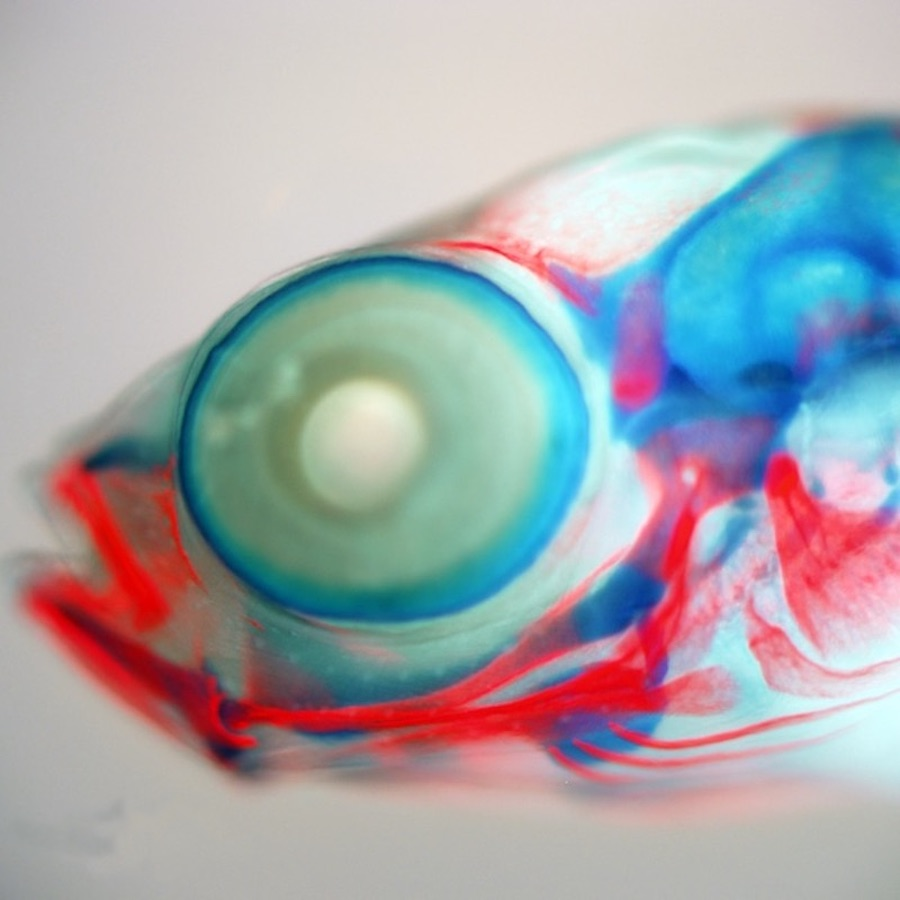
\includegraphics{images/double_head.jpg}
\caption{Photo by Mark Currey}
\end{figure}

\begin{center}\rule{0.5\linewidth}{0.5pt}\end{center}

\hypertarget{fish-density-standards}{%
\section{Fish Density Standards}\label{fish-density-standards}}

(created by M Currey, August 25, 2011, updated by mcc 151125)

These standards for fish densities are what we in the Cresko lab have determined optimal after 12 years of keeping threespine stickleback in a recirculating aquaculture system.

\hypertarget{fry-9dpf---2-months}{%
\subsection{Fry (9dpf - 2 months):}\label{fry-9dpf---2-months}}

• Fry are kept in 2.8 L tanks at an ideal density of 20 fish per container. Fry can be kept in densities of up to 40 fish per tank. If fish densities are near 40 per tank fish are transferred or thinned after 1 month of age.

\hypertarget{juvenile-2-months---4-months-grow-out}{%
\subsection{Juvenile (2 months - 4 months) Grow Out:}\label{juvenile-2-months---4-months-grow-out}}

• Juvenile fish are transferred from fry tanks into 9.5 L tanks and kept at a density of 20 fish per container.

Grow out (4 months -- 1 year), Adult (1 year - 1.5 years) and Breeding conditioning:

• Grow out: Juvenile fish are transferred to 20 gallon tanks in the Winter room at an ideal density of 20 fish per container. Fish can be kept at a density of 40 fish per tank if space is needed.
• Breeding Conditioning: Once fish are 1 year of age (or older), transfer adult fish to the Summer room. Stickleback males become sexually mature 2-6 weeks after experiencing Summer conditions, females become sexually mature 4-6 weeks after experiencing Summer conditions conditions. Conditioned fish can stay in the Summer room for 5 months.

\begin{center}\rule{0.5\linewidth}{0.5pt}\end{center}

\hypertarget{juvenile-collection-daily}{%
\section{Juvenile Collection (Daily):}\label{juvenile-collection-daily}}

\begin{enumerate}
\def\labelenumi{\arabic{enumi}.}
\item
  Turn off water to tanks.
\item
  Remove collection cup, using mysid system water, rinse juveniles into plastic container.
\item
  Pour juveniles into grow out tank.
\item
  Replace collection cup.
\item
  Turn water on and start siphon.
\end{enumerate}

\hypertarget{adult-mysid-collection-and-feeding}{%
\section{Adult mysid collection and feeding:}\label{adult-mysid-collection-and-feeding}}

\begin{enumerate}
\def\labelenumi{\arabic{enumi}.}
\item
  Juvenile will reach adult size in three weeks. At three weeks these new adults will replace old breeding adults. The old breeding adults that are being replaced are feed to the pipefish.
\item
  Let juveniles grow to three weeks at which point they reach adult stage.
\item
  Siphon adults through a net and collect in a container.
\item
  Siphon old adults out of one of the 10 gallon tanks and feed to fish.
\item
  Clean tank, fill with water, and add new adult mysids.
\end{enumerate}

\hypertarget{husbandry-stickleback-health}{%
\chapter{Husbandry stickleback health}\label{husbandry-stickleback-health}}

\begin{figure}
\centering
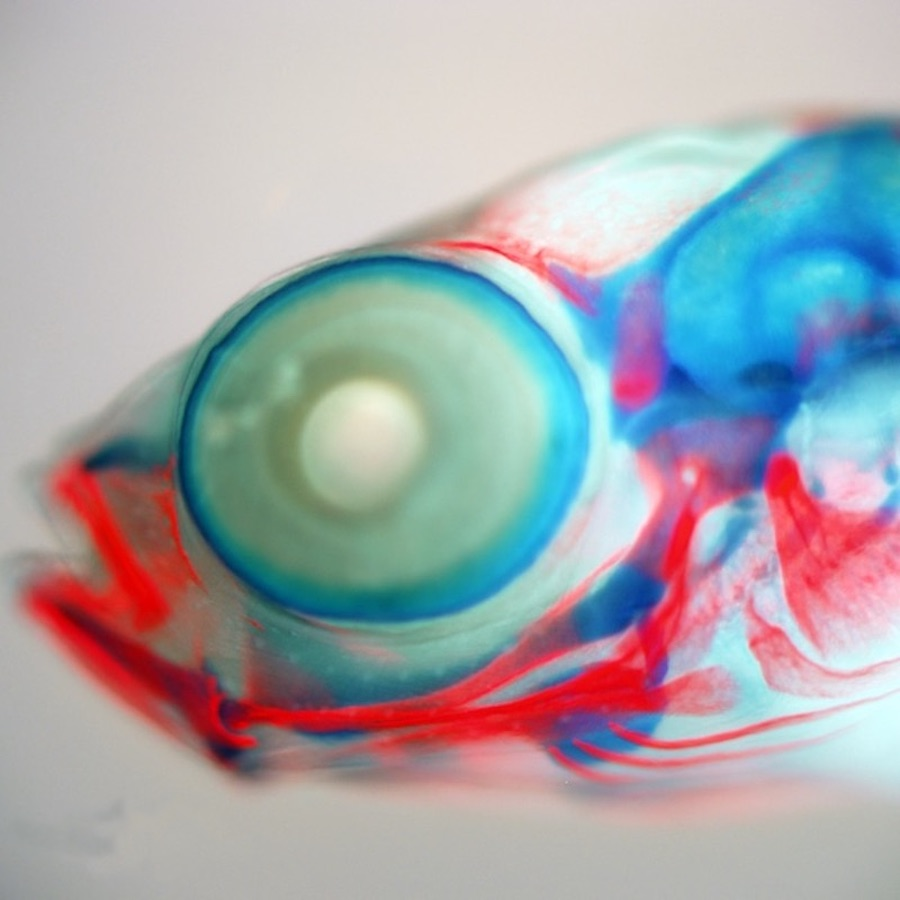
\includegraphics{images/double_head.jpg}
\caption{Photo by Mark Currey}
\end{figure}

\begin{center}\rule{0.5\linewidth}{0.5pt}\end{center}

\hypertarget{health-check---sick-and-dead-fish}{%
\section{Health Check - Sick and Dead Fish}\label{health-check---sick-and-dead-fish}}

(created 4/14/08 by M Currey, updated 151201 by mcc)

*Check for sick and dead fish Daily by looking through all tanks. This is best done when feeding. When done initial checklist and email Mark (see announcement below). Symptoms of Sick and Distressed fish are posted in the fish room.

Material Needed:
• Fish Morgue consisting of a small bucket with lid and a sealable plastic bag
• Mesab, a.k.a. MS222, tricaine or 3-aminobenzoic acid ethyl ester
• Small container
• Net

If dead fish is found:

\begin{enumerate}
\def\labelenumi{\arabic{enumi}.}
\tightlist
\item
  Make note of the number of fish, tank space, and what stock the fish was from on the daily check list.
\item
  With a clean net, remove fish and place into fish morgue. (The fish morgue can be found in the chest freezer. It is a small bucket labeled ``Fish Morgue'' on the lid).
\end{enumerate}

If sick fish is found:

\begin{enumerate}
\def\labelenumi{\arabic{enumi}.}
\tightlist
\item
  Make note on tank and contact supervisor.
\end{enumerate}

Please email Mark with a list of all sick and dead fish along with tank position at the end of each shift, \href{mailto:mcurrey@uoregon.edu}{\nolinkurl{mcurrey@uoregon.edu}}.

If there are numerous sick or dead fish please contact Mark Currey 541-505-0006 or Bill Cresko 541-285-5446 immediately.

\begin{center}\rule{0.5\linewidth}{0.5pt}\end{center}

\hypertarget{adult-fish-anesthesia-euthanasia-and-fixation}{%
\section{Adult fish Anesthesia, Euthanasia, and Fixation}\label{adult-fish-anesthesia-euthanasia-and-fixation}}

(created 4/14/08 by M Currey, updated 151201 by mcc)

** Tricaine must be phamaceutical-grade. (We use tricaine purchased from Aquaic Ecosystems, manufactured by Western Chemical and FDA approved)
These procedures are to be done on fish larger then 5mm in length.

\hypertarget{material-needed}{%
\subsection{Material Needed:}\label{material-needed}}

• Fish Morgue consisting of a small bucket with lid and a sealable plastic bag
• Mesab, a.k.a. MS222, tricaine or 3-aminobenzoic acid ethyl ester
• Small container
• Net

\hypertarget{mesab-stock-solution-4glfrom-zebrafish-book-4th-edition}{%
\subsection{Mesab Stock Solution (4g/L)(From Zebrafish Book 4th edition):}\label{mesab-stock-solution-4glfrom-zebrafish-book-4th-edition}}

Tricaine (3-amino benzoic acid ethy lester also called ethyl m-aminoboenzoate) comes in a powdered form from Sigma (Cat.\# A-5040). It is also available as Finquel (Part No.~C-FINQ-UE) from Argent Chemical Laboratories, Inc.~

\begin{enumerate}
\def\labelenumi{\arabic{enumi}.}
\tightlist
\item
  Make tricaine solution for anesthetizing fish by combining the following in a glass bottle with a screw cap:
\end{enumerate}

• Stock Solution (4g/L)
• 400 mg tricaine powder
• 97.9 ml DD water
• \textasciitilde2.1 ml 1 M Tris (pH 9)

\begin{enumerate}
\def\labelenumi{\arabic{enumi}.}
\setcounter{enumi}{1}
\tightlist
\item
  Adjust pH to \textasciitilde7. Store this solution in the freezer. (Buy the smallest amount possible because tricaine gets old.)
\end{enumerate}

\hypertarget{euthanasia-300-mgl}{%
\subsection{Euthanasia (300 mg/L):}\label{euthanasia-300-mgl}}

Procedure:
1. Make a solution of tris buffered Stock solution MS-222 solution as described above. (Or obtain solution from freezer)
2. Combine 7.5ml of stock solution into 100ml of fish water.
3. Place fish into above fish water/ mesab solution for at least 10 minutes after cessation of opercular movement \textasciitilde12 minutes.
4. If fish is to be used for experiments, proceed with fixation or preparation of the experiment.
5. If the fish are to be disposed of, place fish into fish morgue located in chest freezer in entry room.

\hypertarget{anesthesia-168-mgl}{%
\subsection{Anesthesia (168 mg/L):}\label{anesthesia-168-mgl}}

\begin{enumerate}
\def\labelenumi{\arabic{enumi}.}
\tightlist
\item
  Make a solution of tris buffered Stock solution MS-222 solution as described above. (Or obtain solution from freezer)
\item
  Combine 4.2 ml of stock solution into 100ml of fish water.
\item
  Place fish into 168 mg/l MS-222 solution and wait for the fish to slow down.
\item
  Image or do other experiments quickly to minimize fish exposure to MS-222. Pay attention to opercular movement to be sure that fish is alive.
\item
  Revive by placing in fish water and moving fish gently through the water to pass water over gills.
\end{enumerate}

\hypertarget{liquid-n2-freezing-and-fixation-in-rnalater}{%
\subsection{Liquid N2 freezing, and fixation in RNAlater:}\label{liquid-n2-freezing-and-fixation-in-rnalater}}

\begin{enumerate}
\def\labelenumi{\arabic{enumi}.}
\tightlist
\item
  Anesthetize using above concentration of MS-222 and allow fish to lay motionless with only slight opercle movement. This should take approximately 10 minutes.
\item
  Place fish in liquid N2 for 2 minutes. This instantaneously freezes the fish.
\item
  Thaw into RNAlater-ICE.
\end{enumerate}

SOP - Embryo and Larval Euthanasia and Fixation
(created 4/6/10 by M Currey)

These procedures are to be done with larval fish and fish up to 5mm in length.

For Euthanasia:

Materials:
• Fish Morgue
• Ice bath with basket (see below)
Procedure:
1. Place ice in insulated box, e.g.~cooler or Styrofoam container.
2. Add water to make ice slurry
3. Add mesh basket so that ice water is allowed to enter but ice does not.
4. Place embryos in ice water
5. Let embryos sit for 5 hour minimum
6. Dispose of dead embryos in fish morgue.

For RNA extraction:

Materials:
• RNAlater (Ambion cat \# AM7021) or --80 freezer
• 1.5 ml tubes
• liquid nitrogen

Procedure:
RNA later
1. Add RNA later per manufacturers recommendations.
2. Place embryos in solution. This rapidly fixes embryos.
For Storage in -80° C Freezer
1. Place embryos in 1.5 ml tube
2. Put tube in liquid nitrogen for 2 minutes.
3. Place tube in --80° C for RNA extraction

For insitu hybridization:

Materials:
• 4\% buffered PFA
To make 100 ml of 4\% PFA:
3. Preheat to 60° C while stirring on heat plate
4. Add 4 g PFA
5.\\
Heat and stir just until solution clears. Do not let heat go above 60° C! pH should be about 7.4
6. Store 10ml aliquots at -20C in 1.5 ml tubes

• 1.5 ml tubes
• 10 ml 10XPBS
• 90 ml sterile H2O

Procedure for fixing:
1. Place embryos in 1.5 ml tube
2. Add 1 ml 4\%pfa
3. Store in --20 freezer.
**This rapidly fixes embryos for insitu hybridization.

\hypertarget{husbandry-stickleback-crossing-1}{%
\chapter{Husbandry stickleback crossing}\label{husbandry-stickleback-crossing-1}}

\begin{figure}
\centering
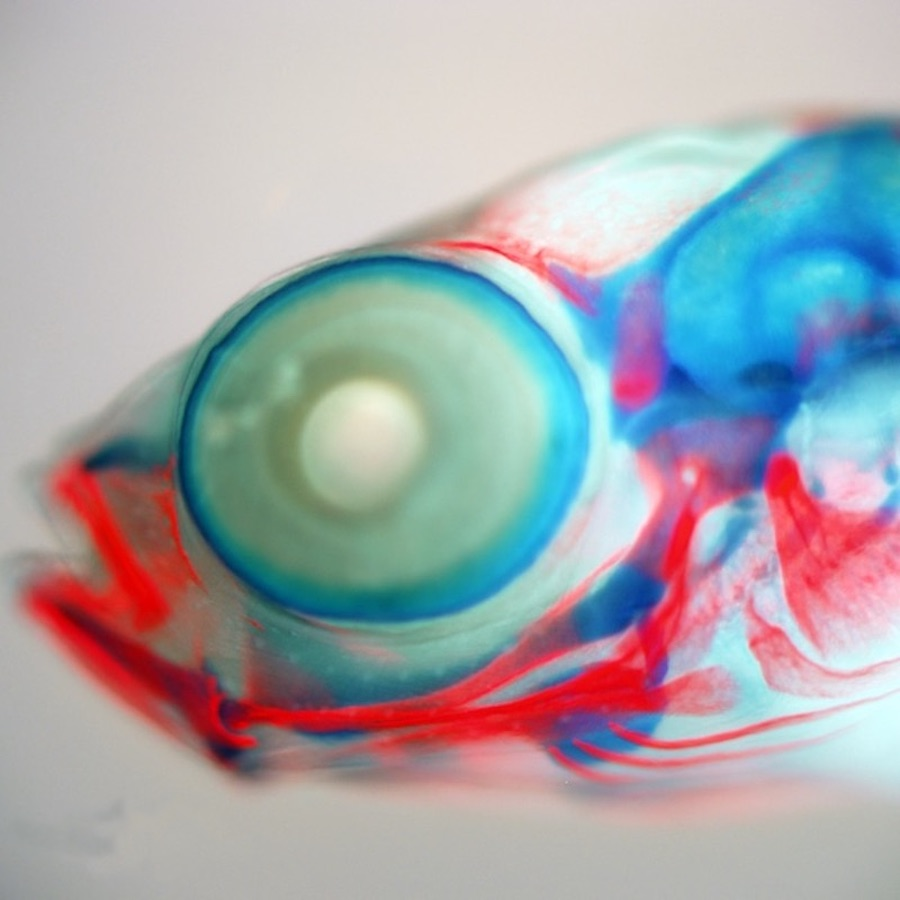
\includegraphics{images/double_head.jpg}
\caption{Photo by Mark Currey}
\end{figure}

\begin{center}\rule{0.5\linewidth}{0.5pt}\end{center}

SOP - Fish Density Standards
(created by M Currey, August 25, 2011, updated by mcc 151125)

These standards for fish densities are what we in the Cresko lab have determined optimal after 12 years of keeping threespine stickleback in a recirculating aquaculture system.

Fry (9dpf - 2 months):

• Fry are kept in 2.8 L tanks at an ideal density of 20 fish per container. Fry can be kept in densities of up to 40 fish per tank. If fish densities are near 40 per tank fish are transferred or thinned after 1 month of age.

Juvenile (2 months - 4 months) Grow Out:

• Juvenile fish are transferred from fry tanks into 9.5 L tanks and kept at a density of 20 fish per container.

Grow out (4 months -- 1 year), Adult (1 year - 1.5 years) and Breeding conditioning:

• Grow out: Juvenile fish are transferred to 20 gallon tanks in the Winter room at an ideal density of 20 fish per container. Fish can be kept at a density of 40 fish per tank if space is needed.
• Breeding Conditioning: Once fish are 1 year of age (or older), transfer adult fish to the Summer room. Stickleback males become sexually mature 2-6 weeks after experiencing Summer conditions, females become sexually mature 4-6 weeks after experiencing Summer conditions conditions. Conditioned fish can stay in the Summer room for 5 months.

\begin{center}\rule{0.5\linewidth}{0.5pt}\end{center}

\hypertarget{embryo-bleaching-for-disinfection}{%
\section{Embryo Bleaching for Disinfection}\label{embryo-bleaching-for-disinfection}}

(created by M Currey, August 25, 2011, updated 151201 by mcc)

\hypertarget{purpose}{%
\subsection{Purpose:}\label{purpose}}

This protocol allows the removal of ecto-parasites from embryos produced from wild-caught stickleback. Use this protocol whenever new fish are added to a pre-existing stickleback rearing system, or whenever stocks are transferred between labs.

\hypertarget{materials-needed}{%
\subsection{Materials needed:}\label{materials-needed}}

• Wash bottle and petri dishes
• Timer

\hypertarget{solutions}{%
\section{Solutions}\label{solutions}}

• 6\% sodium hypochlorite (standard bleach)
• Working stock of bleach -- 500µl of bleach into 1 liter of embryo medium (see rearing protocols)

\hypertarget{procedure}{%
\section{Procedure:}\label{procedure}}

\begin{enumerate}
\def\labelenumi{\arabic{enumi}.}
\item
  Raise embryos according to standard crossing and rearing protocols (see husbandry SOP)
\item
  At 48-60 hours post-fertilization (@ 20C -- at this point most organogenesis is complete) remove embryo medium from petri dishes and rinse embryos once with fresh embryo medium.
\item
  Fill petri dish with working stock solution of bleach. Swirl and let sit for 1.5 min. Do not bleach embryos for longer as chorions can thicken and it becomes difficult for embryos to hatch.
\item
  Drain bleach solution from embryos, and wash them three times with fresh embryo medium. This is really important.
\item
  Replace embryo medium daily. If crosses are done in the field, the embryos can be shipped from day 3 to day 6 post-fertilization. To ship embryos, rinse once with embryo medium, place embryos into a 50ml conical tube (\textasciitilde100 embryos/tube) and fill with fresh embryo medium. Place tubes in a shipping container with wet ice. Separate the tubes from the ice with bubble-wrap and newspapers. Ship the embryos overnight.
\item
  When the embryos arrive at the lab, rinse the outside of the containers well before moving into the lab. Allow them to equilibrate to room temp (\textasciitilde20C). Place the embryos into petri dishes, rinse once, and add new embryo medium. Rear according to standard protocol.
\end{enumerate}

\begin{center}\rule{0.5\linewidth}{0.5pt}\end{center}

\hypertarget{sop-testes-storage}{%
\section{SOP -- Testes Storage}\label{sop-testes-storage}}

(created by M Currey, August 25, 2011, updated 151201 by mcc)

\hypertarget{purpose-storage-of-stickleback-testes-for-fertilization-up-to-1-2-months-post-extraction.}{%
\subsection{Purpose: Storage of stickleback testes for fertilization up to 1-2 months post extraction.}\label{purpose-storage-of-stickleback-testes-for-fertilization-up-to-1-2-months-post-extraction.}}

Materials needed:
• Testes solution
• 15 ml falcon tube
• 4C refrigerator

\hypertarget{procedure-1}{%
\subsection{Procedure:}\label{procedure-1}}

\begin{enumerate}
\def\labelenumi{\arabic{enumi}.}
\tightlist
\item
  Dissect testes (see Stickleback crossing SOP).
\item
  Place testes in 15 ml tube with \textasciitilde{} 10 ml of testes solution.
\item
  Label tube with stock number and date of testes dissection and place tube with testes in 4C refrigerator.
\item
  Change testes solution once per week.
\end{enumerate}

Note: Testes can be used up to \textasciitilde{} 1 month when stored this way.

\begin{center}\rule{0.5\linewidth}{0.5pt}\end{center}

\hypertarget{egg-storage}{%
\section{Egg Storage}\label{egg-storage}}

(created by M Currey, August 25, 2011, updated 151201 by mcc)

\hypertarget{purpose-storage-of-eggs-for-fertilization-up-to-24-hours-post-stripping.}{%
\subsection{Purpose: Storage of eggs for fertilization up to 24 hours post stripping.}\label{purpose-storage-of-eggs-for-fertilization-up-to-24-hours-post-stripping.}}

Materials needed:
• NaCl
• KCl
• CaCl2
• NaHCO3
• Tris, pH 7.2
• npH2O
• Streptomycin \& Penicillin Solution (PenStrep) from Sigma (P-0906) Stock -- 100\%
• 50 ml sterile polypropylene conical tubes
• 90 mm petri dish

\hypertarget{procedure-2}{%
\subsection{Procedure:}\label{procedure-2}}

\begin{enumerate}
\def\labelenumi{\arabic{enumi}.}
\item
  Make stock of Holtfreiter's Solution, store at 4C

  Mix solids into 750ml of npH2O
  3.5 gm NaCl
  0.05 gm KCl
  0.1 gm CaCl2
  0.02 gm NaHCO3
  1.0 ml Tris
  Bring to 1 liter with npH2O
\item
  Add PenStrep to a final concentration of 1\% (10ml into 1 liter), store at 4C.
\item
  Strip eggs from ripe female into a conical tube with 25ml cold Holtfreiters.
\item
  Eggs can be transported on ice and fertilized up to 24 hours later (maybe longer).
\item
  To fertilize, move eggs to 90mm petri dish and allow temperature to equilibrate to 20C.
\item
  Remove Holtfreiter's solution, and rinse eggs once with embryo medium (important to.
  make sure that salt concentration is low enough for sperm to be optimally activated).
\item
  Add macerated testis as in general husbandry SOP and cover eggs with embryo medium.
  SOP - Live Food Culture, Moina and Mysid Shrimp:
  (updated 151201 by mcc)
\end{enumerate}

\begin{center}\rule{0.5\linewidth}{0.5pt}\end{center}

\hypertarget{stickleback-crossing}{%
\section{Stickleback Crossing}\label{stickleback-crossing}}

(Created 4/1/08 by M. Currey)
\#\#\# Materials Needed:
• 25, 45 and 90mm disposable sterile petri dishes (standard)
• Sterile Ginzburg's Fish Ringers solution containing antibiotic and antimycotics for testes (see Testes Solution recipe)
• MS222 Tricaine Methanesulfonate (see Mesab recipe)
• 100\% ethanol
• Fine scissors and forceps
• Wide-blade entomology forceps
• Sterile Embryo medium (6ml of Instant Ocean into 1L npH2O)
• Squeeze wash bottles
• Stress coat (standard from pet store)
• Sterile flat razor blades
• Sterile disposable large bore transfer pipettes (VWR cat\# 691)
• Dissecting microscope

\begin{enumerate}
\def\labelenumi{\arabic{enumi}.}
\tightlist
\item
  Squeeze Female: Cover fingers with stress coat and gently squeeze gravid female. Gravid females have extended abdomens and their eggs have ``dropped''. If eggs do not emerge with very slight pressure the female is not quite ready. Squeeze eggs with motion from pectoral girdle posterior to the cloaca into a 25mm sterile petri dish. The small size of petri dish allows the sperm to be concentrated on the eggs.
\item
  Dissect Testes From Male: Euthanize male by placing him into a finger bowl of embryo medium containing a lethal volume of MS222. Clean a large, 30cm by 60cm or similar size, glass sheet, fine scissors, and forceps with 100\% ethanol. When male is motionless, remove and rinse fish with clean water and sever spinal cord behind skull using a razor to be sure of euthanization. Use scissors to make incision just posterior to the cloaca and cut from there anteriorly to the pelvic girdle making an incision along the mid line of the fish. Make another cut to each side of the fish from the cloaca dorsally approximately 15mm so that the body cavity is easily accessed. Incisions should be made just deep enough to cut the skin and body wall muscle while being wary to not cut into the stomach and intestines that are located just below the skin surface. Locate paired testes and vas deferens (testes are variable in shape and coloration, but are usually long and pigmented, usually having the same pigmentation as the skin surface, and sit in the dorsal part of the coelom near the kidneys. The vas deferens are threadlike and are usually as long as the testis to which it connects. Use fine forceps to grab vas deferens, sever near the cloaca, and remove one (or often) both testes. Doing so keeps the testes intact, allowing them to contain viable sperm for up to 1 month at 4°C in Testes Solution.
\item
  Storing of Testes: If only a single cross is to be made with a male, proceed to step 4. Otherwise, place testes into 45mm petri dish filled with cold Testes Solution. Store testes at 4°C. To store testes for extended periods, change out medium once a week.
\item
  Prepare Testis: If multiple crosses are to be performed from a single pair of male's testes, remove one testis and place on the inside lid of the 25mm petri dish into which a females eggs have been squeezed. Using a sterile razor, slice off a small piece of testis (we've found a large testis can be used to fertilize approximately 5 clutches). Make cuts as perpendicular as possible to the major axis of the testis and perform multiple cuts from the same end. This allows as much of the sperm to remain packaged and inactivated at the center of the testis. Use blade to macerate testis. Under a dissecting scope swimming sperm should cause a `sparkling' refraction. Add approximately 1.0 ml of sterile embryo medium to testis prep with disposable pipette, mix, and then add to the eggs one drop at a time, using same disposable pipette, dispersing drops between petri dishes so that all eggs are covered with sperm mixture.
\item
  Fertilization (time = 0): Fertilization of most eggs will occur almost instantaneously. However, I leave the sperm on the eggs for about 5-10 minutes. At this point cover embryos with embryo medium. Mark fertilization time (this is the time that the initial drops of sperm were added) on the surface of the petri dish. Place in incubator at 20°C.
\item
  Separation of Embryos and Second Cleaning (t = 2 hr): The animal pole of the embryo is established at the site of sperm entry, and at 20°C the first cell syncitium is usually visible within 45 minutes. The first cell division usually occurs approximately 25 minutes later, and the two cell stage is fully visible approximately 1.5hr after fertilization. During this time, the chorion thickens and attaches to the petri dish as well as to other embryos. At or after 2 hours post fertilization, use the wide blade entomological forceps to detach the embryos from one another, as well as to dislodge embryos from the bottom of the petri dish. Remove all of the unfertilized eggs to limit mold contamination, and record the total number of eggs and embryos. Rinse embryos 3 to 4 more times then distribute embryos to 90mm petri dishes (30-50 embryos per dish) filled half way with fresh embryo medium. Enter cross information into database, print labels for dishes, and place embryos into incubator at 20°C.
\item
  Raise Embryos (check daily): Embryos will develop at approximately 2.5 times zebrafish time {[}see \url{http://zfin.org/zf_info/zfbook/stages/index.html}{]}, and hatch at approximately 7 days. 48hr stickleback embryos have completed most major morphogenetic processes, and the melanic pigment cells are just starting to migrate. A beating heart can be seen after \textasciitilde72hr. Check petri dishes daily and remove those that have arrested development. A change of embryo medium may help at some point during the first 7 days as water quality may decline.
\end{enumerate}

\begin{center}\rule{0.5\linewidth}{0.5pt}\end{center}

\hypertarget{incubator-use-and-care-of-stickleback-fry}{%
\section{Incubator Use and Care of Stickleback Fry}\label{incubator-use-and-care-of-stickleback-fry}}

(Created 4/1/08 by M. Currey)

\hypertarget{purpose-1}{%
\subsection{Purpose:}\label{purpose-1}}

Researchers are responsible for monitoring and caring of their research animals while in the incubator. This includes water changes, removing ``deads'', fixing, euthanizing and any other procedures regarding the fish. If the fish are to be raised past hatching please contact Mark, prior to hatching, to make arrangements for putting fish into system. Also, please see Mark prior to initial use of incubator for brief training.

\hypertarget{materials-needed-1}{%
\subsection{Materials needed:}\label{materials-needed-1}}

• Petri Dishes
• Embryo Medium (found above incubator)
• Incubator
• Fry food
• checklist

\hypertarget{procedure-3}{%
\subsection{Procedure:}\label{procedure-3}}

Raise Embryos (check daily):
Embryos will develop at approximately 2.5 times zebrafish time {[}see \url{http://zfin.org/zf_info/zfbook/stages/index.html}{]}, and hatch at approximately 7 days. 48hr stickleback embryos have completed most major morphogenetic processes, and the melanic pigment cells are just starting to migrate. A beating heart can be seen after \textasciitilde72hr. Check petri dishes daily and remove deads and those with arrested development. A change of embryo medium may help at some point during the first 7 days as water quality may decline.

Hatching, Begin Feeding Brine Shrimp, and Move to System (t = 7-8 days post fertilization): After hatching at 7-8 days post fertilization, remove chorions and allow young to absorb yolk (2-3 days). At approximately day 2 post hatching take petri dish containing fry out of incubator and place dishes on a table. To each petri dish add approximately the same volume of system water, as there is embryo medium; this will double the volume of liquid in the dish. This acclimates the fry to the system water. Allow the fry to acclimate for 6-10 hours, the longer the better. Then transfer fry to small aquaria on the system. Feed newly hatched brine shrimp once daily and fry food once daily according to directions posted in the fish room.

• Initial checklist and add what type of check was done to checklist.

\hypertarget{husbandry_stickleback_food}{%
\chapter{Husbandry\_stickleback\_food}\label{husbandry_stickleback_food}}

\begin{figure}
\centering
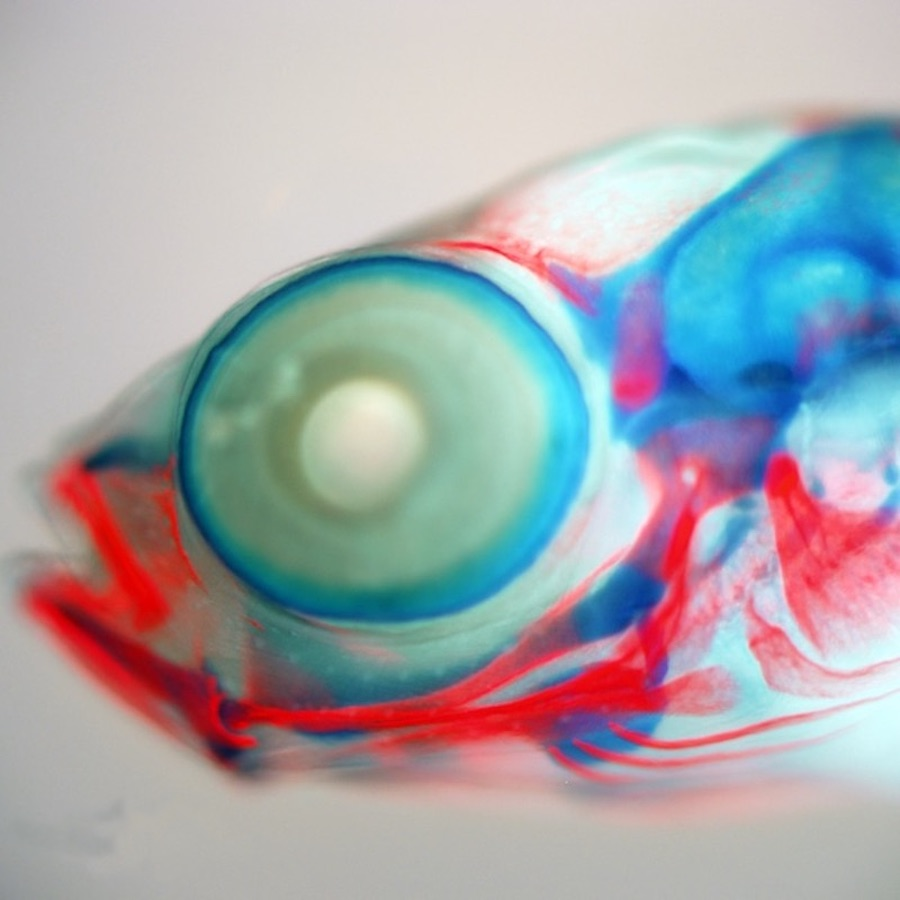
\includegraphics{images/double_head.jpg}
\caption{Photo by Mark Currey}
\end{figure}

\begin{center}\rule{0.5\linewidth}{0.5pt}\end{center}

\hypertarget{stickleback-feeding}{%
\section{Stickleback Feeding}\label{stickleback-feeding}}

(created May 6, 2008 by m currey, revised October 21, 2014 by mcc)

\hypertarget{materials}{%
\subsection{Materials:}\label{materials}}

\begin{itemize}
\tightlist
\item
  Fish food mix or dry fry food
\item
  Decapsulated Artemia (see artemia decapsulating SOP)
\item
  Color coded feeding Spoon
\end{itemize}

\hypertarget{fish-foods-for-fry-and-juvenileadults}{%
\subsection{Fish foods for fry and juvenile/adults:}\label{fish-foods-for-fry-and-juvenileadults}}

\begin{itemize}
\tightlist
\item
  Fry - newly hatched baby brine shrimp (see hatching brine shrimp SOP) and Zeigler Larval Diet (Larva ``Z'' Plus 250-450 Microns).
\item
  Juvenile and Adult fish food mix (see fish food mix SOP).
\end{itemize}

\emph{Dry Foods Are Stored in freezer in the stickleback facility}

\emph{Procedure:}
- Fry are located along the south wall of the summer room.
- AM feeding: Feed fry once per day with newly hatched brine shrimp (this should happen during the opposite feeding of larval diet)
- PM feeding: Feed fry once per day with Ziegler larval diet 1/8 spoon full.
- Juvenile and Adults are located in the 20 gallon tanks in the Summer and Winter rooms. Additionally, individualized adults are sometimes located on the fry rack in the Summer room. Please check white board for notification of adults on fry rack.
- Feed juveniles and adults twice per day with dry food mix. Using the color coding on spoon, food mix, and tags on tanks. (e.g.~for adults: use the red spoon, red food mix, and feed the tanks with a red tag).
- Unused brine shrimp can be fed to juvenile and adult fish.

\hypertarget{food-storage-and-handling}{%
\subsection{Food Storage and Handling:}\label{food-storage-and-handling}}

\begin{itemize}
\tightlist
\item
  See Fish food storage SOP.
\end{itemize}

\emph{Initial daily check list after you have fed. }

\begin{center}\rule{0.5\linewidth}{0.5pt}\end{center}

\hypertarget{fish-food-mix}{%
\section{Fish Food Mix}\label{fish-food-mix}}

(created August 25, 2011 m currey)

\hypertarget{materials-1}{%
\subsection{Materials:}\label{materials-1}}

\begin{itemize}
\tightlist
\item
  Freezer
\item
  Fridge
\item
  1 gallon bucket with a tight seal
\item
  plastic measuring cup
\end{itemize}

\hypertarget{dry-mix}{%
\subsection{Dry Mix:}\label{dry-mix}}

\begin{itemize}
\tightlist
\item
  Mix the following dry foods in 1 gallon bucket
\end{itemize}

\hypertarget{juvenile-mix}{%
\subsection{Juvenile Mix:}\label{juvenile-mix}}

\begin{itemize}
\tightlist
\item
  4 cups Pentair finfish starter ZC1
\item
  1 cup New Life Spectrum optimum saltwater flake
\item
  1 cup Ziegler AP100
\end{itemize}

\hypertarget{adult-mix}{%
\subsection{Adult mix:}\label{adult-mix}}

\begin{itemize}
\tightlist
\item
  4 cups Pentair finfish starter ZP1
\item
  4 cups Pentair finfish starter ZC1
\item
  1 cup New Life Spectrum grow
\item
  1 cup New Life Spectrum optimum saltwater flake
\item
  1 cup Hikari micro pellet
\item
  1 cup Hikari marine S
\item
  1/8 cup golden pearls
\end{itemize}

\hypertarget{storage}{%
\subsection{Storage:}\label{storage}}

\begin{itemize}
\tightlist
\item
  Label with expiration date (6 months after making) and store at -20°C.
\end{itemize}

\begin{center}\rule{0.5\linewidth}{0.5pt}\end{center}

\hypertarget{fish-food-storage-and-sources}{%
\section{Fish Food: Storage and Sources}\label{fish-food-storage-and-sources}}

(created by M Currey, August 25, 2011)

\emph{Label all foods with received date and expiration date
(see below for how to determine expiration date).}

\hypertarget{brine-shrimp}{%
\subsection{Brine Shrimp:}\label{brine-shrimp}}

Good indefinitely if frozen in tightly sealed container

1 Upon receiving label with received date.
Store unopened tins in -20°C freezer.
After de-capsulation label with date de-capsulated and date of expiration (30 days from de-capsulation).
Store de-capsulated shrimp at 4°C.

Source -- Brine Shrimp Direct, www.brineshrimpdirect.com

\hypertarget{golden-pearl-larval-diet}{%
\subsection{Golden Pearl Larval Diet:}\label{golden-pearl-larval-diet}}

\begin{enumerate}
\def\labelenumi{\arabic{enumi}.}
\tightlist
\item
  800 -- 1000 micron
\end{enumerate}

Good 3-5 years if kept in freezer

\begin{enumerate}
\def\labelenumi{\arabic{enumi}.}
\tightlist
\item
  Store in -20°C freezer.
\item
  Unopened label with expiration date 3 years from receiving date.
\item
  Upon opening change expiration date to 6 months from date opened.
\end{enumerate}

Source -- Brine Shrimp Direct, www.brineshrimpdirect.com

\hypertarget{hikari-dry-foods}{%
\subsection{Hikari dry foods:}\label{hikari-dry-foods}}

• Marine S
• Micro Pellets

If un-opened, expiration date is labeled on container by manufacturer. Once opened the food is good for 6 months.

\begin{enumerate}
\def\labelenumi{\arabic{enumi}.}
\tightlist
\item
  Keep out of direct sunlight, high heat, and humidity.
\item
  Store at 4°C.
\item
  Upon opening change expiration date to 6 months from date opened.
\end{enumerate}

Source -- Pet Mountain, www.petmountain.com
That Pet Place: \url{http://www.thatpetplace.com}

New Life Spectrum dry foods:

\begin{enumerate}
\def\labelenumi{\arabic{enumi}.}
\setcounter{enumi}{1}
\tightlist
\item
  Optimum saltwater flakes
\item
  Growth Formula
\end{enumerate}

If un-opened, expiration date is labeled on container by manufacturer. Once opened the food is good for 6 months.

• Keep out of direct sunlight, high heat, and humidity.
• Store at 4°C.
• Upon opening change expiration date to 6 months from date opened.

Source -- Jehmco, www.jehmco.com

\hypertarget{zeigler-larval-dry-food}{%
\subsection{Zeigler Larval dry food:}\label{zeigler-larval-dry-food}}

\begin{enumerate}
\def\labelenumi{\arabic{enumi}.}
\tightlist
\item
  AP100 (150-250 microns)
\end{enumerate}

Good 2 years if kept unopened and in freezer.

• Upon receiving label with received date and expiration date (2 years from received date).
• Store at 4°C.
• Upon opening change expiration date to 6 months from date opened.

Source -- Aquatic Ecosystems, \url{http://pentairaes.com}
Pentair Finfish Starter dry foods:

\begin{enumerate}
\def\labelenumi{\arabic{enumi}.}
\setcounter{enumi}{1}
\tightlist
\item
  ZP1 - 1.5 mm slow sinking pellet
\item
  ZC1 -- 0.6 -- 0.85 mm \#1 crumble
\end{enumerate}

If un-opened, expiration date is labeled on container by manufacturer. Once opened the food is good for 6 months.

• Keep out of direct sunlight, high heat, and humidity.
• Store at 4°C.
• Upon opening change expiration date to 6 months from date opened.

Source -- Aquatic Ecosystems, \url{http://pentairaes.com}

\hypertarget{selcon-brine-shrimp-supplement}{%
\subsection{Selcon (brine shrimp supplement):}\label{selcon-brine-shrimp-supplement}}

Good 1 year if kept unopened and in fridge.

\begin{enumerate}
\def\labelenumi{\arabic{enumi}.}
\tightlist
\item
  Upon receiving label with received date and expiration date (1 years from received date).
\item
  Store at 4°C.
\end{enumerate}

Source -- Aquatic Ecosystems, \url{http://www.aquaticeco.com/}

\hypertarget{frozen-mysid-and-blood-worms}{%
\subsection{Frozen Mysid and Blood Worms:}\label{frozen-mysid-and-blood-worms}}

Expiration date printed on front label.

\begin{itemize}
\tightlist
\item
  Upon receiving label with received.
\item
  Store at -20°C.
\end{itemize}

Source -- Nautilus Tropical Fish -- Springfield Oregon, 727 Main St.~541-344-3474

\begin{center}\rule{0.5\linewidth}{0.5pt}\end{center}

\hypertarget{hatching-and-feeding-brine-shrimp}{%
\section{Hatching and Feeding Brine Shrimp}\label{hatching-and-feeding-brine-shrimp}}

(created by M Currey 5/6/08, updated 151201 mcc)

\hypertarget{materials-needed-2}{%
\subsection{Materials Needed:}\label{materials-needed-2}}

\begin{itemize}
\tightlist
\item
  De-capsulated Brine Shrimp
\item
  Rock Salt
\item
  105 μm mesh shrimp collector
\item
  Baking Soda
\item
  Squirt Bottle
\end{itemize}

\hypertarget{procedure-4}{%
\subsection{Procedure:}\label{procedure-4}}

\begin{enumerate}
\def\labelenumi{\arabic{enumi}.}
\tightlist
\item
  Collect Brine Shrimp: Drain entire cone into 105 μm mesh shrimp collector (located on shelf near cone). Rinse and pour shrimp into squirt bottle. Feed fish. Rinse squirt bottle and place on shelf to dry.
\item
  Reset Brine Cone: Fill cone with DI water to 10 L. Put airline and heater (set at 80°F) into cone. Add 300 ml of rock salt and 1 scoop (5 ml) of baking soda. Obtain de-capsulated brine from refrigerator and shake to homogenize solution. Measure out 150 ml* of de-capsulated brine and add it to the cone.
\item
  Wait 24 hours and repeat\ldots.
\end{enumerate}

\begin{itemize}
\tightlist
\item
  The amount of brine shrimp needed will vary depending on the number of juvenile fish that need to be fed. If there is a need for more brine shrimp add more de-capsulated brine to cone and leave a note for the next person. Increase the amount in 50 ml increments. *
\end{itemize}

\begin{center}\rule{0.5\linewidth}{0.5pt}\end{center}

\hypertarget{artemia-decapsualtion}{%
\section{Artemia Decapsualtion}\label{artemia-decapsualtion}}

(Adapted by M Currey 4/3/08, 151201 updated by mcc)

\hypertarget{materials-2}{%
\subsection{Materials:}\label{materials-2}}

\begin{itemize}
\tightlist
\item
  15 oz can of dried Artemia cysts (approximately 430 g)
\item
  4.3 L \textasciitilde6\% laundry grade bleach
\item
  Rock Salt (NaCl)
\item
  125 ml 40\% Lye (NaOH) solution
\item
  30.0 g Sodium thiosulfate (Na2S2O3)
\item
  16 L Hatching Cone with aeration
\item
  125 μm mesh bag (Aquatic Eco-Systems PMB3, 125 micron x 18")
\item
  Several 3-5 L beakers
\item
  (1-2) Squirt bottles - squeeze type
\end{itemize}

\hypertarget{solutions-1}{%
\section{Solutions:}\label{solutions-1}}

\begin{itemize}
\item
  Solutions should be prepared in advance *
\item
  Bleach, \textasciitilde6\% laundry grade
\item
  25 ppt Salt Solution:
\end{itemize}

\begin{enumerate}
\def\labelenumi{\arabic{enumi}.}
\tightlist
\item
  Combine: 50 g Rock Salt (NaCl) To 2.0 L with tap water
\item
  Stir to dissolve completely.
\end{enumerate}

\begin{itemize}
\tightlist
\item
  40\% Lye (NaOH) solution
\end{itemize}

\begin{enumerate}
\def\labelenumi{\arabic{enumi}.}
\tightlist
\item
  Combine: 200 g Lye (NaOH) To 500 mL with tap water
\item
  Stir to dissolve completely.
\item
  Store in refrigerator (4°C)
\end{enumerate}

\begin{itemize}
\tightlist
\item
  Buffered Salt Solution
\end{itemize}

\begin{enumerate}
\def\labelenumi{\arabic{enumi}.}
\tightlist
\item
  Combine: 2L, 25 ppt Salt Solution
\item
  125 mL 40\% Lye Solution, pre-chilled to 4°C
\end{enumerate}

\begin{itemize}
\tightlist
\item
  1.0\% Sodium Thiosulfate
\end{itemize}

\begin{enumerate}
\def\labelenumi{\arabic{enumi}.}
\tightlist
\item
  Combine: 30 g sodium thiosulfate To 3.0 L with tap water
\item
  Stir to dissolve.
\end{enumerate}

\begin{itemize}
\tightlist
\item
  Saturated Brine
\end{itemize}

\begin{enumerate}
\def\labelenumi{\arabic{enumi}.}
\tightlist
\item
  Combine: \textasciitilde25g Rock Salt to 4.0 L with tap water
\item
  Aerate to dissolve.
\end{enumerate}

\hypertarget{procedure-5}{%
\subsection{Procedure:}\label{procedure-5}}

\begin{enumerate}
\def\labelenumi{\arabic{enumi}.}
\tightlist
\item
  Cyst hydration: Hydrate one full can of dried cyst in 5 L of tap water in a hatching cone with aeration for 1 hour at room temp. Examine the cyst under a dissecting scope with top lighting before proceeding. Dry cysts are dimpled, resembling a deflated basketball, whereas fully hydrated cysts are completely spherical in shape. The cysts must be fully hydrated prior to the de-capsulation step. If cysts are not completely spherical after 1 hour, continue the hydration process (for a maximum of 2 hours), checking the progress of the cysts under a microscope every 15 min.
\item
  Filter and rinse cysts: Collect the hydrated cyst in a 125 um mesh bag and rinse with cool tap water.
\item
  Transfer cysts back to the cone: Add the Buffered Salt Solution to the cone and aerate (save back a filled squirt bottle of salt solution to help transfer cysts to cone). Transfer cysts into cone.
\item
  De-capsulation: Add the bleach (4.3 L) to the cone and continue aeration. Watch the cysts turn from brown to grey to orange, When the cysts are 90\% orange, stop the reaction by quickly siphoning the cysts through a 125 um mesh bag and rinsing well with cool tap water.
\item
  Neutralization residual chlorine: To neutralize any residual chlorine transfer the mesh bag to a clean 4 L beaker and pour the 1.0\% Sodium Thiosulfate (3L) into the bag. Soak the cysts in the sodium thiosulfate solution for \textasciitilde1 min, then rinse the cysts with de-ionized tap water. Rinse until discharge turns clear.
\item
  Dehydration for long-term storage: Transfer the cysts back to the cone with 4 L of saturated brine and aerate until salt is dissolved. Transfer dehydrated cyst to (5 or 6) 1 L Nalgene bottles filled with 200 - 300 grams of salt. Add enough salt so that it does not dissolve when de-capsulated brine is added. Fill the bottles with de-capsulated brine. Store in refrigerator. The de-capsulated brine will store for at least 1 month. Hatch brine as you would capsulated brine (see Hatching and Feeding Brine SOP).
\end{enumerate}

\begin{center}\rule{0.5\linewidth}{0.5pt}\end{center}

\hypertarget{moina}{%
\section{Moina}\label{moina}}

Materials:
• 10 gallon glass tanks
• corner sponge filter
• Air supply
• Rotifer diet
• Powdered nannochloropsis

\hypertarget{procedure-6}{%
\subsection{Procedure:}\label{procedure-6}}

\begin{enumerate}
\def\labelenumi{\arabic{enumi}.}
\tightlist
\item
  Fill 10 gallon tank 3/4 full of stickleback system water
\item
  Add corner filter and activate with air.
\item
  Add Moina
\item
  Change water once every 2-3 weeks by removing half of the water and replacing with stickleback water.
\item
  DO NOT break tank down and clean as moina do not respond well to this.
\end{enumerate}

\hypertarget{feeding}{%
\subsection{\texorpdfstring{\textbf{Feeding}:}{Feeding:}}\label{feeding}}

\begin{enumerate}
\def\labelenumi{\arabic{enumi}.}
\setcounter{enumi}{5}
\tightlist
\item
  Add 15 drops of rotifer diet and 1/8 scoop of powdered nannochloropsis each day.
\end{enumerate}

\hypertarget{mysid-shrimp}{%
\section{Mysid Shrimp}\label{mysid-shrimp}}

For a description of the mysid generator please visit:
\url{http://www.mblaquaculture.com/assets/docs/MBL_AQ_Mysid_Generator.pdf}

\hypertarget{materials-3}{%
\subsection{Materials:}\label{materials-3}}

• 10 gallon tank generator system
• Salt water

\hypertarget{feeding-1}{%
\subsection{Feeding:}\label{feeding-1}}

\begin{enumerate}
\def\labelenumi{\arabic{enumi}.}
\tightlist
\item
  Feed newly hatched brine shrimp daily to both adults and juveniles.
\end{enumerate}

\hypertarget{water-change}{%
\subsection{Water Change:}\label{water-change}}

\begin{enumerate}
\def\labelenumi{\arabic{enumi}.}
\tightlist
\item
  2-3 times per week empty 5 gallons of water from the system and replace with new make up water.
\item
  Make new water in 5 gallon bucket by adding DI water and 2 scoops of salt.
\end{enumerate}

\hypertarget{husbandry_stickleback_food-1}{%
\chapter{Husbandry\_stickleback\_food}\label{husbandry_stickleback_food-1}}

\begin{figure}
\centering
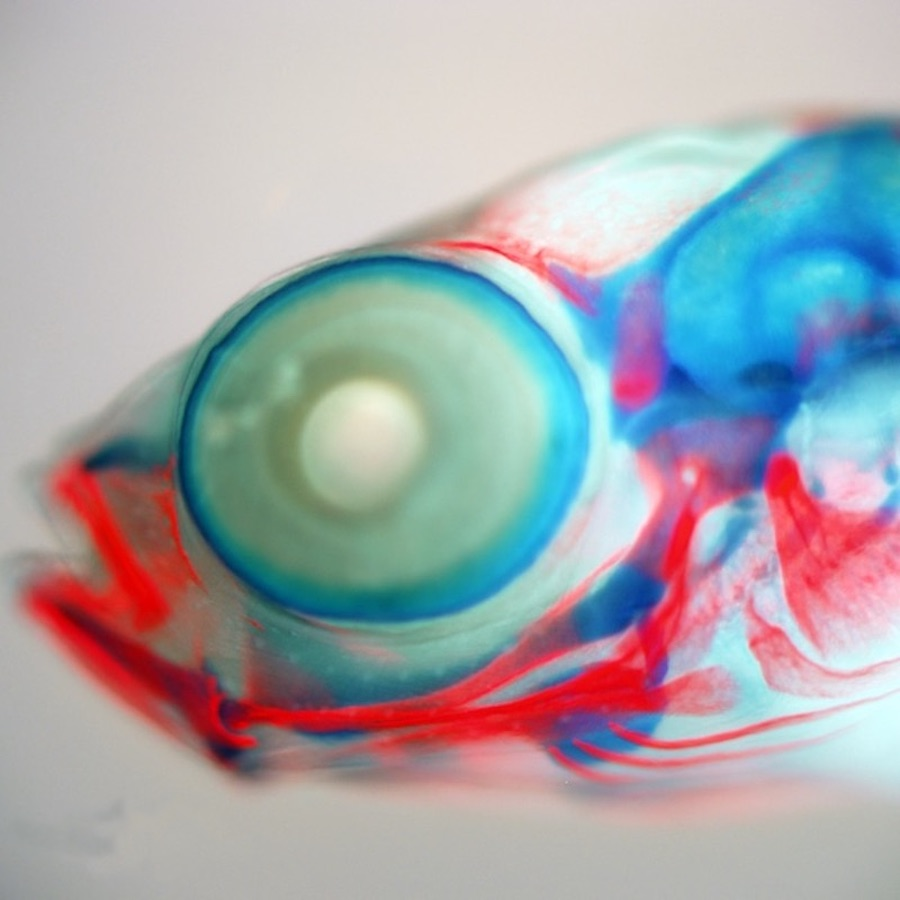
\includegraphics{images/double_head.jpg}
\caption{Photo by Mark Currey}
\end{figure}

\begin{center}\rule{0.5\linewidth}{0.5pt}\end{center}

\hypertarget{gallon-tank-cleaning}{%
\section{20 gallon Tank Cleaning}\label{gallon-tank-cleaning}}

(Created April 8, 2008 by M. Currey, revised March 3, 2012 by M. Currey)

\textbf{\emph{Tank cleaning is to be done ONLY during the week}}

\hypertarget{material-needed-1}{%
\subsection{Material needed:}\label{material-needed-1}}

• Household bleach in a squirt bottle
• Scrub pad or sponge
• Siphon tip
• Siphon hose
• Portable waste water collector
• Scrubber pads
• Scrubber handles
• Cart (you may or may not want to use)
• Old clothes (this can be messy)
• Personal protection equipment (Splash proof glasses or face shield).

\begin{enumerate}
\def\labelenumi{\arabic{enumi}.}
\tightlist
\item
  Siphon (cleaning by ``vacuuming'') Attach siphon tip onto siphon hose. The siphon tips, which are attached to the hoses, are the only parts of this apparatus that can be immersed in the tank. Start siphon by running system water into hose until hose is filled with water. Turn valve so that water is ``trapped'' in hose. Put end of tip into tank that is being cleaned and turn valve back on creating a siphon. Vacuum all waste off of the bottom being careful to not suck up any fish. Use each tip in only one tank and then sterilize it by washing in the dishwasher (see Dishwasher SOP).
\item
  Scrubbing (removal of algae from sides, front, and back of tank) is done on an ``as needed'' basis. (If you can't see into the tank, it's past time to scrub.) With a Scotch Brite Pad (United Grocers, Eugene, Oregon) scrub front and sides of tank. Do not use pad on multiple tanks. Autoclave scrubber pads to sterilize.
\item
  Replace basket of bulkhead. Take the dirty basket off and sterilize in dishwasher as described above. Obtain clean basket and replace.
\end{enumerate}

Note: When using bleach and/or sodium thiosulfate. Eye protection is required. Please use splash proof glasses or a face shield when using bleach and sodium thiosulfate.

\begin{enumerate}
\def\labelenumi{\arabic{enumi}.}
\setcounter{enumi}{3}
\tightlist
\item
  Complete bleaching and cleaning of tank. This needs to be done to each tank every 2 months. Remove fish from tank and put them into a clean tank. Tanks that are emptied of fish need to be cleaned and sterilized before another batch of fish can be introduced. Drain the tank and remove it from the rack. Clean all parts with brushes and a scrub pad or put into the bleach bin. Clean the tank thoroughly with a scrub pad, taking care not to damage the silicon water seals on the inside (algae should be left if very gentle rubbing will not remove it. Squirt about 10 -- 20 mls of bleach into the tank. Wash the bleach water thoroughly around the inside of the tank by hand, using a pad, sponge, tank back, or other means to expose all inside portions of the tank to bleach. Rinse the tank thoroughly with hot tap water. Rinse the tank with sodium thiosulfate, and then rinse it again with hot water. Put a few thiosulfate crystals into the tank and leave it. Reassemble the tank and put it back on the rack. Fill with system water and allow water to recirculate for about 30 minutes before adding fish. Watch fish for 15min to look for any signs of distress.
\item
  Initial check list
\end{enumerate}

\begin{center}\rule{0.5\linewidth}{0.5pt}\end{center}

\hypertarget{corner-filter-cleaning}{%
\section{Corner filter cleaning:}\label{corner-filter-cleaning}}

\hypertarget{procedure-7}{%
\subsection{Procedure:}\label{procedure-7}}

\begin{enumerate}
\def\labelenumi{\arabic{enumi}.}
\tightlist
\item
  Remove dirty corner filters from tanks and rinse with tap water to remove excess algae and debris.
\item
  Put corner filters inside bleack tank and leave them soaking over night.
\item
  Rinse the corner filters with hot water for 5 min being sure to fill and dump the filter with water at least 5 times and then place them into the sodium thiosulfate tank rinse out with the sodium thiosulfate solution 2 times and leave them to soak overnight.
\item
  Rinse the corner filters for 5 minutes repeating the fill and dump method as above with hot water, and leave them drying on the rack overnight.
\item
  When cleaned corner filters are placed back into aquaria, observe fish for 15 min for signs of distress.
\end{enumerate}

\begin{center}\rule{0.5\linewidth}{0.5pt}\end{center}

\hypertarget{fry-tank-cleaning}{%
\section{Fry Tank Cleaning}\label{fry-tank-cleaning}}

(Created 4/10/08 by M Currey)

Fish put into fry tanks will live in these tanks for 2-3 months at which point the tank will be emptied and sterilized using the dishwasher then stored for further use. If the fry remain in these tanks for longer then 3 months, or there is a build-up of waste or algae in the tanks, then follow the following procedure.

\hypertarget{materials-needed-3}{%
\subsection{Materials Needed:}\label{materials-needed-3}}

• 2.8 L or 9.5 L aquaneering tanks
• matching lid
• fry baffle note: When placing new fish into the system use 400 micron (smaller) mesh baffles.

\hypertarget{procedure-8}{%
\subsection{Procedure:}\label{procedure-8}}

\begin{enumerate}
\def\labelenumi{\arabic{enumi}.}
\tightlist
\item
  Obtain clean fry tank and install lid and baffle.
\item
  Put fish from dirty tank into clean tank. To do this remove dirty fish tank from rack and carefully pour off 1/3 of tank water. Then pour the rest of the water and fish into clean tank. If there is lots of waste in the tank transfer fish with a net to leaving waste in dirty tank.
\item
  Put clean tank of fish back on rack and start water.
\end{enumerate}

\begin{center}\rule{0.5\linewidth}{0.5pt}\end{center}

\hypertarget{dishwasher-use-to-sterilize-plastics-and-glassware}{%
\section{Dishwasher use to sterilize plastics and glassware}\label{dishwasher-use-to-sterilize-plastics-and-glassware}}

(created 4/2016 by J. Crandall)

\hypertarget{loading-the-dishwasher}{%
\subsection{Loading the dishwasher:}\label{loading-the-dishwasher}}

\begin{verbatim}
If there are clean dishes from a previous cycle, put them away in their respective locations. If some are still wet, set them out to dry on the drying rack before putting them away. 
RINSE ALL DIRTY DISHES VERY WELL, especially those with algae/food residue. the dishwasher will sanitize, but will not effectively clean, the dishes. Scrub dishes with a scrub pad to remove buildup, if needed. 
Tank tube and bulkhead pieces should be hung on the vertical rinsing pipes on the bottom rack; longer tank tubes should be placed on the top rack if they would impede the rinser on the bottom of the top rack from spinning. 
Small tank lids should be stacked on the bottom rack, but not on the raised portion of the rack, as this impedes the rinser from spinning properly.
Plastic tanks, Ziploc containers and long tank tubes should be placed on the top rack.
\end{verbatim}

\textbf{BEFORE RUNNING THE DISHWASHER, SLIDE BOTH RACKS IN AND MAKE SURE THE RINSER ON THE BOTTOM OF THE TOP RACK CAN SPIN FREELY}

\hypertarget{running-the-dishwasher}{%
\subsection{Running the dishwasher:}\label{running-the-dishwasher}}

\begin{verbatim}
Add ~1/2 scoop of dish detergent (found under the sink) to the well in the door of the dishwasher. Close the lid to the well.
Close and latch the door to the dishwasher. The display will light up, and after booting up it should read “User 1.” Press the RUN/CANCEL button to begin the cycle. If it instead displays a list of programs, use the down arrow key to navigate down the list to “User 1.” When the “User 1” program is highlighted, press the RUN/CANCEL button to begin the cycle. If the screen displays something other than “User 1,” press the DISPLAY button to show the list of programs, scroll down to “User 1,” and press RUN/CANCEL.  
Should the program ever need to be cancelled mid-cycle, pressing the RUN/CANCEL button once will result in the cycle canceling and the water draining. 
\end{verbatim}

\hypertarget{large-tank-lids}{%
\subsection{Large tank lids:}\label{large-tank-lids}}

• The small frontal lids to the large glass tanks should be loaded into the dishwasher. The large lids to the large glass tanks should be hosed off thoroughly with very hot water, and set on the rack to dry.

\hypertarget{recipes}{%
\chapter{Recipes}\label{recipes}}

\begin{figure}
\centering
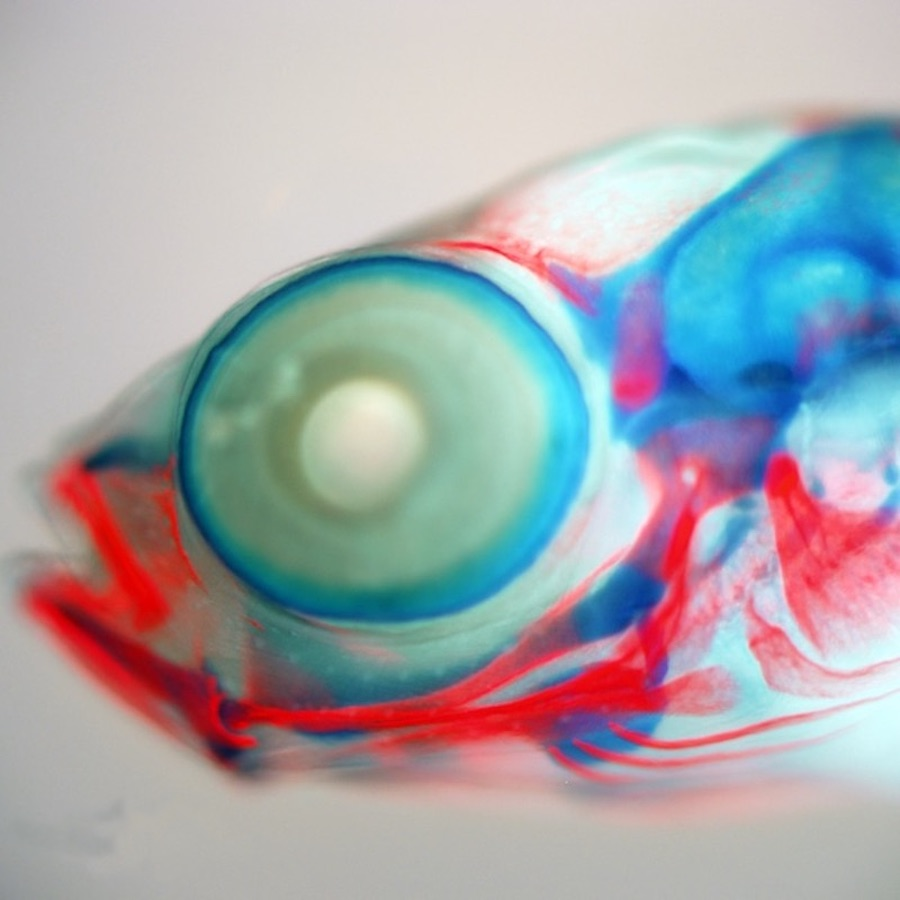
\includegraphics{images/double_head.jpg}
\caption{Photo by Mark Currey}
\end{figure}

\begin{center}\rule{0.5\linewidth}{0.5pt}\end{center}

\hypertarget{embryo-medium}{%
\section{Embryo Medium}\label{embryo-medium}}

\hypertarget{material-needed-2}{%
\subsection{Material Needed:}\label{material-needed-2}}

\begin{itemize}
\tightlist
\item
  Instant Ocean Salt
\item
  Baking Soda
\item
  npH2O
\end{itemize}

\hypertarget{embryo-medium-solution}{%
\subsection{Embryo Medium solution:}\label{embryo-medium-solution}}

\begin{enumerate}
\def\labelenumi{\arabic{enumi}.}
\tightlist
\item
  Add 8g Instant Ocean to 2 liters of npH2O
\item
  Add \textasciitilde0.5g baking soda
\item
  Check pH and adjust to 7.0 -- 8.0
\item
  This makes 2 liters
\end{enumerate}

\begin{itemize}
\tightlist
\item
  Salt and baking soda are located in containers near the dissecting scope. Rinse 2 liter flasks with DI water between uses.
  \_\_\_\_\_\_\_\_\_\_\_\_\_
\end{itemize}

\hypertarget{mesab}{%
\section{MESAB}\label{mesab}}

\emph{Tricaine must be pharmaceutical-grade. We use tricaine purchased from Pentair, manufactured by Western Chemical and FDA approved. Tricaine (3-amino benzoic acid ethyl lester also called ethyl m-aminoboenzoate) comes in a powdered form. Purchase the smallest amount possible because tricaine expires quickly.}

\hypertarget{material-needed-3}{%
\subsection{Material Needed:}\label{material-needed-3}}

\begin{itemize}
\tightlist
\item
  Mesab, a.k.a. MS222, tricaine, or 3-aminobenzoic acid ethyl ester
\item
  1 M Tris (pH 9)
\item
  DD water
\end{itemize}

\hypertarget{mesab-stock-solution-4gl-tris-buffered}{%
\subsection{Mesab Stock Solution (4g/L) (tris buffered):}\label{mesab-stock-solution-4gl-tris-buffered}}

\begin{itemize}
\item
  \begin{enumerate}
  \def\labelenumi{\arabic{enumi}.}
  \tightlist
  \item
    4 g tricaine powder
  \end{enumerate}
\item
  \begin{enumerate}
  \def\labelenumi{\arabic{enumi}.}
  \setcounter{enumi}{1}
  \tightlist
  \item
    979 ml DD water
  \end{enumerate}
\item
  \textasciitilde21 ml 1 M Tris (pH 9)
\item
  Adjust pH to \textasciitilde7\\
\item
  Aliquot in 50ml tubes, label with MESAB Stock Solution 4g/L, and store in a -20 freezer
\item
  This makes 1 liter of solution.
\end{itemize}

\hypertarget{euthanasia-solution-300-mgl}{%
\subsection{Euthanasia Solution (300 mg/L):}\label{euthanasia-solution-300-mgl}}

\begin{enumerate}
\def\labelenumi{\arabic{enumi}.}
\tightlist
\item
  Make a solution of tris buffered Stock Solution as described above. (Or obtain an aliquot from the freezer)
\item
  Combine 7.5ml of stock solution into 100 ml of fish water.
\end{enumerate}

\hypertarget{anesthesia-168-mgl-1}{%
\subsection{Anesthesia (168 mg/L):}\label{anesthesia-168-mgl-1}}

\begin{enumerate}
\def\labelenumi{\arabic{enumi}.}
\tightlist
\item
  Make a solution of tris buffered Stock Solution as described above. (Or obtain an aliquot from the freezer)
\item
  Combine 4.2 ml of stock solution into 100 ml of fish water.
\end{enumerate}

\begin{center}\rule{0.5\linewidth}{0.5pt}\end{center}

\hypertarget{testes-storage-solution}{%
\section{Testes Storage Solution}\label{testes-storage-solution}}

\hypertarget{materials-needed-4}{%
\subsection{Materials Needed:}\label{materials-needed-4}}

\begin{enumerate}
\def\labelenumi{\arabic{enumi}.}
\tightlist
\item
  NaCl
\item
  KCl
\item
  CaCl2
\item
  NaHCO3
\item
  npH2O
\item
  Gentamycin (antimycotic) (Stock -- 10mg/ml)*
\item
  Cell Culture anti-biotic/mycotic from Gibco-BRL (15240-096) 100x Concentration*.
\end{enumerate}

\begin{itemize}
\tightlist
\item
  Both of these reagents are located in separate boxes in Mark's space in the
\item
  20° C freezer. They are partitioned into 100μl aliquots.
\end{itemize}

\hypertarget{solutions-2}{%
\subsection{Solutions:}\label{solutions-2}}

Ginzberg's Ringers
- Mix solids into 750 ml of npH2O
- 6.6g NaCl
- 0.25g KCl
- 0.3g CaCl2
- 0.2g NaHCO3
- Bring to 1 liter total volume with npH2O.
- Store at 4° C.

\hypertarget{testes-solution-100ml}{%
\subsection{Testes solution (100ml)}\label{testes-solution-100ml}}

• Add 100μl of Gentamycin and 100μl of Anti-biotic/mycotic to 100ml of Ginzburg's Ringers solution.
• Store at 4° C.

\hypertarget{pipefish-husbandry-protocols}{%
\chapter{Pipefish Husbandry Protocols}\label{pipefish-husbandry-protocols}}

\begin{figure}
\centering
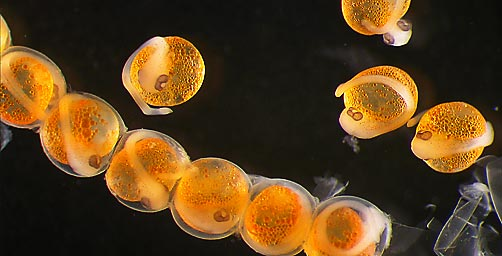
\includegraphics{images/pipefish_embryos.jpg}
\caption{Photo by Mark Currey}
\end{figure}

\begin{center}\rule{0.5\linewidth}{0.5pt}\end{center}

\hypertarget{pipefish-feeding}{%
\section{Pipefish Feeding}\label{pipefish-feeding}}

(created by M Currey 7/23/09)

\textbf{Materials Needed:}

\begin{itemize}
\item
  Decapsualted Brine Shrimp (see artemia decapsulations SOP)
\item
  Adult Brine Shrimp
\item
  Live Moina
\item
  Frozen myisid Shrimp
\item
  Live mysid shrimp
\item
  Shrimp collector
\item
  Squirt Bottle
\item ~
  \hypertarget{fish-foods-for-fry-juvenile-and-adults}{%
  \subsection{Fish foods for fry, juvenile and adults:}\label{fish-foods-for-fry-juvenile-and-adults}}
\item
  Fry - newly hatched baby brine shrimp (see hatching brine shrimp SOP), salt water copepods. Fry are fed once per day
\item
  Adult -- newly hatched brine shrimp, Adult brine shrimp, Moina. Adults are fed once per day. Feed adult brine shrimp when we have them. Use moina when we are out of adult brine shrimp. Adult brine shrimp are from a local fish store and are only available every tow weeks. They last \textasciitilde{} one week and therefore adult pipefish are fed adult brine shrimp for one week and moina the next.
\end{itemize}

\textbf{Fry:}

\begin{verbatim}
     Fry tanks are designated with an orange dot. 
\end{verbatim}

\begin{enumerate}
\def\labelenumi{\arabic{enumi}.}
\tightlist
\item
  Newly hatched brine: Collect newly hatched brine and place into a squirt bottle (see brine shrimp SOP). Feed all tanks with an orange dot.
\end{enumerate}

\textbf{Adults:}

\begin{verbatim}
    Adult tanks are designated with a yellow dot. 
\end{verbatim}

\begin{enumerate}
\def\labelenumi{\arabic{enumi}.}
\tightlist
\item
  Newly hatched brine: Collect newly hatched brine and place into a squirt bottle (see brine shrimp SOP). Feed all tanks with an orange dot.
\item
  Frozen Mysis: Obtain a quarter-sized piece of frozen mysis from the freezer. Place into squirt bottle and add water. Wait until mysis thaws and feed to all adult tanks.
\item
  Adult Brine shrimp: Scoop out adult brine shrimp with net. Wash into a ball and place over the top of squirt bottle. Wash ball of brine into squirt bottle and feed all adult pipefish.
\item
  Moina: Scoop out with net and wash into a ball. Invert ball over collection beaker and wash moina into beaker. Pour moina into squirt bottle and feed.
\item
  Live Mysid: See live foods SOP
\end{enumerate}

\hypertarget{live-food-culture-monia-and-mysid-shrimp}{%
\section{\texorpdfstring{\textbf{Live Food Culture, Monia and Mysid Shrimp:}}{Live Food Culture, Monia and Mysid Shrimp:}}\label{live-food-culture-monia-and-mysid-shrimp}}

\textbf{\emph{Moina}}

\textbf{Materials:}

\begin{itemize}
\tightlist
\item
  10 gallon glass tanks
\item
  corner sponge filter
\item
  Air supply
\item
  Rotifer diet
\item
  Powdered nannochloropsis
\end{itemize}

\textbf{Procedure:}

\begin{itemize}
\tightlist
\item
  Fill 10 gallon tank 3/4 full of stickleback system water
\item
  Add corner filter and activate with air.
\item
  Add Moina
\item
  Change water once every 2-3 weeks by removing half of the water and replacing with stickleback water.
\item
  DO NOT break tank down and clean as moina do not respond well to this.
\end{itemize}

\textbf{Feeding:}

\begin{itemize}
\tightlist
\item
  Add 15 drops of rotifer diet and 1/8 scoop of powdered nannochloropsis each day.
\end{itemize}

\hypertarget{collection-and-feeding-to-fish}{%
\subparagraph{Collection and feeding to fish}\label{collection-and-feeding-to-fish}}

\begin{itemize}
\tightlist
\item
  See pipefish feeding SOP
\end{itemize}

\hypertarget{mysid-shrimp-1}{%
\subparagraph{\texorpdfstring{\emph{Mysid Shrimp}}{Mysid Shrimp}}\label{mysid-shrimp-1}}

For a description of the mysid generator please visit:

\url{http://www.mblaquaculture.com/assets/docs/MBL_AQ_Mysid_Generator.pdf}

\textbf{Materials:}

\begin{itemize}
\tightlist
\item
  10 gallon tank generator system
\item
  Salt water
\end{itemize}

\textbf{Feeding:}

\begin{itemize}
\tightlist
\item
  Feed newly hatched brine shrimp daily to both adults and juveniles.
\end{itemize}

\textbf{Water Change:}

\begin{itemize}
\tightlist
\item
  2-3 times per week empty 5 gallons of water from the system and replace with new make up water.
\item
  Make new water in 5 gallon bucket by adding DI water and 2 scoops of salt.
\end{itemize}

\textbf{Juvenile Collection (Daily):}

\begin{itemize}
\tightlist
\item
  Turn off water to tanks.
\item
  Remove collection cup, using mysid system water, rinse juveniles into plastic container.
\item
  Pour juveniles into grow out tank.
\item
  Replace collection cup.
\item
  Turn water on and start siphon.
\end{itemize}

\textbf{Adults collection and feeding to pipefish:}

Juvenile will reach adult size in three weeks. At three weeks these new adults will replace old breeding adults. The old breeding adults that are being replaced are feed to the pipefish.

\begin{itemize}
\tightlist
\item
  Let juveniles grow to three weeks at which point they reach adult stage
\item
  Siphon adults through a net and collect in a container.
\item
  Siphon old adults out of one of the 10 gallon tanks and feed to pipefish
\item
  Clean tank, fill with water and add new adult.
\end{itemize}

\newpage

\hypertarget{live-food-culture-monia-and-mysid-shrimp-1}{%
\section{Live Food Culture, Monia and Mysid Shrimp:}\label{live-food-culture-monia-and-mysid-shrimp-1}}

\textbf{\emph{Moina}}

\textbf{Materials:}

\begin{itemize}
\tightlist
\item
  10 gallon glass tanks
\item
  corner sponge filter
\item
  Air supply
\item
  Rotifer diet
\item
  Powdered nannochloropsis
\end{itemize}

\textbf{Procedure:}

\begin{itemize}
\tightlist
\item
  Fill 10 gallon tank 3/4 full of stickleback system water
\item
  Add corner filter and activate with air.
\item
  Add Moina
\item
  Change water once every 2-3 weeks by removing half of the water and replacing with stickleback water.
\item
  DO NOT break tank down and clean as moina do not respond well to this.
\end{itemize}

\textbf{Feeding:}

\begin{itemize}
\tightlist
\item
  Add 15 drops of rotifer diet and 1/8 scoop of powdered nannochloropsis each day.
\end{itemize}

\hypertarget{collection-and-feeding-to-fish-1}{%
\subparagraph{Collection and feeding to fish}\label{collection-and-feeding-to-fish-1}}

\begin{itemize}
\tightlist
\item
  See pipefish feeding SOP
\end{itemize}

\hypertarget{mysid-shrimp-2}{%
\subparagraph{\texorpdfstring{\emph{Mysid Shrimp}}{Mysid Shrimp}}\label{mysid-shrimp-2}}

For a description of the mysid generator please visit:

\url{http://www.mblaquaculture.com/assets/docs/MBL_AQ_Mysid_Generator.pdf}

\textbf{Materials:}

\begin{itemize}
\tightlist
\item
  10 gallon tank generator system
\item
  Salt water
\end{itemize}

\textbf{Feeding:}

\begin{itemize}
\tightlist
\item
  Feed newly hatched brine shrimp daily to both adults and juveniles.
\end{itemize}

\textbf{Water Change:}

\begin{itemize}
\tightlist
\item
  2-3 times per week empty 5 gallons of water from the system and replace with new make up water.
\item
  Make new water in 5 gallon bucket by adding DI water and 2 scoops of salt.
\end{itemize}

\textbf{Juvenile Collection (Daily):}

\begin{itemize}
\tightlist
\item
  Turn off water to tanks.
\item
  Remove collection cup, using mysid system water, rinse juveniles into plastic container.
\item
  Pour juveniles into grow out tank.
\item
  Replace collection cup.
\item
  Turn water on and start siphon.
\end{itemize}

\textbf{Adults collection and feeding to pipefish:}

Juvenile will reach adult size in three weeks. At three weeks these new adults will replace old breeding adults. The old breeding adults that are being replaced are feed to the pipefish.

\begin{itemize}
\tightlist
\item
  Let juveniles grow to three weeks at which point they reach adult stage
\item
  Siphon adults through a net and collect in a container.
\item
  Siphon old adults out of one of the 10 gallon tanks and feed to pipefish
\item
  Clean tank, fill with water and add new adult.
\end{itemize}

\hypertarget{histological-protocols}{%
\chapter{Histological Protocols}\label{histological-protocols}}

\hypertarget{alizarin-staining}{%
\section{Alizarin Staining}\label{alizarin-staining}}

\hypertarget{purpose-alizarin-staining-of-fixed-adult-stickleback.}{%
\subsection{PURPOSE: Alizarin staining of fixed adult stickleback.}\label{purpose-alizarin-staining-of-fixed-adult-stickleback.}}

\hypertarget{materials-4}{%
\subsection{MATERIALS:}\label{materials-4}}

\begin{itemize}
\tightlist
\item
  0.5\% Alizarin red S Stock: To make 50 mls add 0.25g alizarin red S powder to 50 ml water.
\item
  0.025\% Alizarin Stain: To make 100 mls: Add 500µl 0.5\% alizarin red S (stock) to 99.5ml 1\% KOH
\item
  1 Liter: Add 5ml 0.5\% alizarin red S (stock) to 9950ml (1 liter) 1\%KOH
\item
  3\% H202/0.5\%KOH: Mix and keep at 4C; Before using, bring to room temperature to hold down
\item
  introducing bubbles under the skin: 0.5ml 6\%H202 \& 0.5ml 1\%KOH.
\item
  MESAB: Tricaine: 3-amino benzoic acid ethyl ester from Sigma (Cat \# A-5040). Mix in fish safe container with a stir bar:

  \begin{itemize}
  \tightlist
  \item
    400 mg tricaine powder
  \item
    800 mg Na2HPO4 (anhydrous)
  \item
    100 ml glass distilled water
  \end{itemize}
\end{itemize}

Adjust to \textasciitilde pH 7 with a drop at a time of 1N NaOH or 1N HCl if needed
but it's usually right if you weigh the sodium phosphate carefully and
measure the water with a graduated cylinder.

For storage: Aliquot into 6 x 25 ml fish safe plastic bottles and store
at 4C. Label with date made and use within a couple of weeks.

8\% PFA: \{\#pfa .subhead2\}

\begin{itemize}
\tightlist
\item
  8 g Pelleted PFA (Ted Pella, Inc.; cat\# 18501)
\item
  90 ml dH2O
\item
  25 drops 1N NaOH
\end{itemize}

\begin{enumerate}
\def\labelenumi{\arabic{enumi}.}
\tightlist
\item
  Heat at very low heat and stir until solution clears.
\item
  Add 25 drops 1N HCl. pH should be 7.0-7.2.
\item
  Filter and store at 4C not more than 1 week.
\item
  Use as 4\% PFA: dilute 1:1 with 2X PBS, do not store solution more
  than a few hours.
\end{enumerate}

2X PBS \{\#x-pbs .subhead2\}

\begin{itemize}
\tightlist
\item
  1.6\% NaCl
\item
  0.04\% KCl
\item
  0.04 M PO4 pH 7.0- 7.3
\end{itemize}

\hypertarget{procedure-9}{%
\subsection{Procedure:}\label{procedure-9}}

Day

Step

Time for Step

Date and Time

1

2h-8h at R/T depending on size on shaker.

1h or longer at R/T on shaker.

Without agitation and with lid open until eyes start to lighten and all
skin pigment is gone (usually about an hour or more)

2

2 h to O/N at R/T on shaker

2 h to overnight O/N at R/T on shaker.\\
Check for bone staining.

R/T on shaker until excess stain in tissue is gone.

Without agitation

Wild caught specimens are put in 100\% EtOH in the field and then
rehydrated and put into 4\% when back in the lab.

\hypertarget{iacuc}{%
\chapter{IACUC}\label{iacuc}}

descriptions of animal care IACUC protocols

  \bibliography{book.bib,packages.bib}

\end{document}
